\documentclass[11pt]{article}
\usepackage[margin=1in]{geometry}
\usepackage[T1]{fontenc}
\usepackage{lmodern}
\usepackage{microtype}
\usepackage{booktabs}
\usepackage{array}
\usepackage{longtable}
\usepackage{tabularx}
\usepackage{adjustbox}
\usepackage{xcolor}
\usepackage{tikz}
\usetikzlibrary{arrows.meta,positioning,calc,fit,backgrounds}
\definecolor{linkblue}{HTML}{1F4E79}
\definecolor{softred}{HTML}{B23A48}
\definecolor{softgreen}{HTML}{2E7D32}
\definecolor{softgray}{HTML}{666666}
\setlength{\parindent}{0pt}
\setlength{\parskip}{0.6em}

\title{A Stakeholder-Aware CEO Playbook}
\author{}
\date{}

\begin{document}
\maketitle
\thispagestyle{empty}

This note turns the classic ``drastic changes'' table into a compact decision model.
Each executive action is represented in three ways:
(1) as a business action,
(2) as a set of COCOMO-style driver changes, and
(3) as a source of stakeholder tension.

\section*{1. Stakeholder space}
Stakeholders are located in a four-dimensional space using a five-point scale.
At one end of each dimension is a lightweight, local preference; at the other is a more strategic or controlling preference.

\begin{table}[h!]
\centering
\small
\begin{tabular}{lcc}
\toprule
Dimension & 0 & 4 \\
\midrule
Now     & Now      & Later \\
Build   & Use      & Build \\
Change  & Stable   & Change \\
Control & Autonomy & Control \\
\bottomrule
\end{tabular}
\caption{Stakeholder dimensions (0--4 scale).}
\end{table}

\begin{table}[h!]
\centering
\small
\begin{tabular}{lcccc}
\toprule
Group & Now & Build & Change & Control \\
\midrule
Users       & 0 & 0 & 1 & 0 \\
Customers   & 1 & 0 & 1 & 2 \\
Developers  & 1 & 4 & 3 & 0 \\
QA          & 2 & 2 & 1 & 3 \\
Managers    & 3 & 2 & 2 & 4 \\
Executives  & 4 & 3 & 4 & 4 \\
Regulators  & 4 & 0 & 0 & 4 \\
Ops         & 1 & 3 & 0 & 2 \\
\bottomrule
\end{tabular}
\caption{Canonical stakeholder groups in the 4D space.}
\end{table}

An organization is modeled as a weighted mix of at most three groups, e.g. customers:developers:executives = 1:2:2.
Its organizational preference vector is the weighted centroid of those groups.

\section*{2. Drastic actions and the knobs that implement them}
The action table should not be bland.  Each row should say what an executive move means in operational terms.
The table below keeps the spirit of the original: each drastic business action is tied to concrete driver changes.

\begin{table}[h!]
\centering
\scriptsize
\begin{adjustbox}{max width=\textwidth}
\begin{tabular}{>{\raggedright\arraybackslash}p{0.03\textwidth} >{\raggedright\arraybackslash}p{0.34\textwidth} >{\raggedright\arraybackslash}p{0.58\textwidth}}
\toprule
\# & Drastic change & Effects (COCOMO drivers pushed) \\
\midrule
1 & Improve personnel
  & acap=5; pcap=5; pcon=5; aexp=5; plex=5; ltex=5 \\
2 & Improve tools, techniques, or development platform
  & tool=5; time=3; stor=3; pvol=2; site=6 \\
3 & Improve precedentedness / development flexibility
  & prec=5; flex=5 \\
4 & Increase architectural analysis / risk resolution
  & resl=5 \\
5 & Relax schedule
  & sced=5 \\
6 & Improve process maturity
  & pmat=5 \\
7 & Reduce functionality
  & data=2; cplx=2 \\
8 & Improve the team
  & team=5 \\
9 & Reduce quality
  & rely=1; docu=1; time=3; cplx=1 \\
\bottomrule
\end{tabular}
\end{adjustbox}
\caption{Implementing drastic changes via driver settings.}
\end{table}

\section*{3. The same actions seen as social tensions}
Every action also has a political signature.
For each row, there is some group most likely to welcome the move and some group most likely to resist it.
That opposition can be summarized as a main tension in the 4D space.

\begin{table}[h!]
\centering
\scriptsize
\begin{adjustbox}{max width=\textwidth}
\begin{tabular}{c p{0.26\textwidth} p{0.19\textwidth} p{0.19\textwidth} p{0.22\textwidth}}
\toprule
\# & Action & Most likes & Most hates & Main tension \\
\midrule
1 & Improve personnel & Executives, managers & Staff, unions, weak performers & Control vs Autonomy \\
2 & Improve tools / platform & Architects, innovators & Legacy maintainers, conservative ops & Change vs Stability \\
3 & Improve precedentedness / flexibility & Strategists, R\&D & Regulators, fixed-plan customers & Change vs Control \\
4 & Increase risk analysis & QA, architects, regulators & Developers under delivery pressure & Control vs Autonomy \\
5 & Relax schedule & Developers, QA & Sales, impatient customers & Build vs Use \\
6 & Improve process maturity & QA, managers, auditors & Developers, agile teams & Control vs Autonomy \\
7 & Reduce functionality & Developers, maintainers & Customers, sales, product owners & Build vs Use \\
8 & Improve the team & Leadership, strong contributors & Politically entrenched or low performers & Control vs Comfort \\
9 & Reduce quality & Short-term sales, speed-focused executives & Users, QA, support & Now vs Later \\
\bottomrule
\end{tabular}
\end{adjustbox}
\caption{Each action is also a stakeholder conflict.}
\end{table}

\section*{4. Decision rule}
We optimize for:
\emph{minimize change, maximize delivered value, minimize effort, and minimize risk}.
But an action is not acceptable just because it scores well on those objectives.
An action may still trigger alarms if it moves too close to a group's negative concerns.

A simple model is:
\[
\textit{score}(a)=w_1\,\textit{change}(a)+w_2\,\textit{effort}(a)+w_3\,\textit{risk}(a)-w_4\,\textit{value}(a)
\]
for action $a$, subject to stakeholder constraints:
\[
\textit{pain}(g,a) \le \tau_g \quad \text{for each stakeholder group } g
\]
where $\tau_g$ is that group's tolerance threshold.
In words: choose good actions, but reject actions that make some constituency scream too loudly.

\section*{5. A single killer figure}
Figure~\ref{fig:killer} ties the whole story together.
An executive chooses an action.
That action changes concrete project drivers.
Those driver changes produce objective consequences (cost, effort, risk, value) and social consequences (who likes it, who hates it).
The chosen decision is therefore not just ``the best'' move; it is the best move that does not trigger unacceptable alarms.

\begin{figure*}[t]
\centering
\tiny
\linespread{0.92}\selectfont
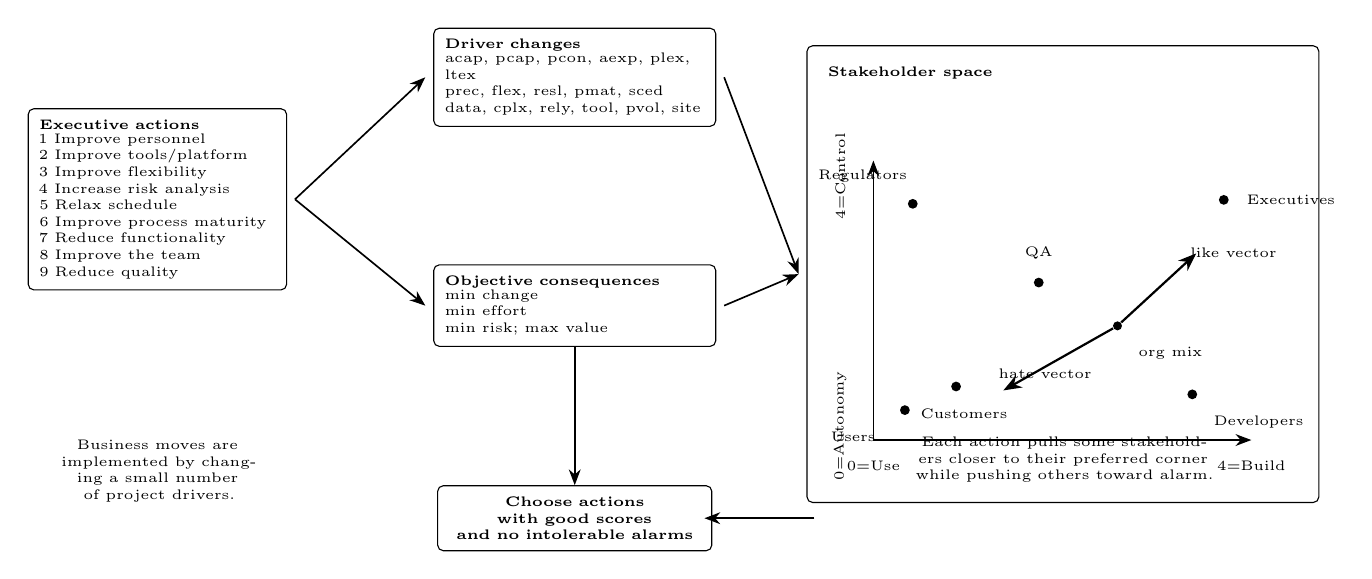
\begin{tikzpicture}[
  >=Stealth,
  every node/.style={font=\tiny},
  box/.style={draw, rounded corners=2pt, align=left, inner sep=4pt},
  arr/.style={->, semithick}
]

%--------------------------------------------------
% left: executive actions
%--------------------------------------------------
\node[box, text width=3.0cm] (actions) at (0,0) {
\textbf{Executive actions}\\[-1pt]
1 Improve personnel\\
2 Improve tools/platform\\
3 Improve flexibility\\
4 Increase risk analysis\\
5 Relax schedule\\
6 Improve process maturity\\
7 Reduce functionality\\
8 Improve the team\\
9 Reduce quality
};

\node[align=center, text width=2.7cm] at (0,-3.45) {
Business moves are implemented by changing a small number of project drivers.
};

%--------------------------------------------------
% middle top: driver changes
%--------------------------------------------------
\node[box, text width=3.3cm] (drivers) at (5.3,1.55) {
\textbf{Driver changes}\\[-1pt]
acap, pcap, pcon, aexp, plex, ltex\\
prec, flex, resl, pmat, sced\\
data, cplx, rely, tool, pvol, site
};

%--------------------------------------------------
% middle bottom: objective consequences
%--------------------------------------------------
\node[box, text width=3.3cm] (obj) at (5.3,-1.35) {
\textbf{Objective consequences}\\[-1pt]
min change\\
min effort\\
min risk; max value
};

%--------------------------------------------------
% bottom center: decision rule
%--------------------------------------------------
\node[box, align=center, text width=3.2cm] (choose) at (5.3,-4.05) {
\textbf{Choose actions with good scores}\\
\textbf{and no intolerable alarms}
};

%--------------------------------------------------
% right: stakeholder space
%--------------------------------------------------
\node[box, minimum width=6.5cm, minimum height=5.8cm] (space) at (11.5,-0.95) {};
\node[anchor=north west] at ([xshift=1.5mm,yshift=-1.5mm]space.north west) {\textbf{Stakeholder space}};

% plot origin and axes
\coordinate (o) at ([xshift=0.85cm,yshift=0.8cm]space.south west);
\draw[arr] (o) -- ++(4.8,0);
\draw[arr] (o) -- ++(0,3.55);

% axis endpoint labels
\node[below=4pt] at (o) {0=Use};
\node[below=4pt] at ($(o)+(4.8,0)$) {4=Build};
\node[rotate=90] at ($(o)+(-0.42,0.18)$) {0=Autonomy};
\node[rotate=90] at ($(o)+(-0.42,3.35)$) {4=Control};

% stakeholder points
\node[circle,fill,inner sep=1.25pt,
      label={[xshift=-2mm,yshift=-1mm]below left:Users}] 
      (u) at ($(o)+(0.40,0.38)$) {};

\node[circle,fill,inner sep=1.25pt,
      label={[xshift=1mm,yshift=-1mm]below:Customers}] 
      (c) at ($(o)+(1.05,0.68)$) {};

\node[circle,fill,inner sep=1.25pt,
      label={[xshift=1mm,yshift=-1mm]below right:Developers}] 
      (d) at ($(o)+(4.05,0.58)$) {};

\node[circle,fill,inner sep=1.25pt,
      label={[yshift=1mm]above:QA}] 
      (q) at ($(o)+(2.10,2.00)$) {};

\node[circle,fill,inner sep=1.25pt,
      label={[xshift=1mm]right:Executives}] 
      (e) at ($(o)+(4.45,3.05)$) {};

\node[circle,fill,inner sep=1.25pt,
      label={[xshift=1mm,yshift=1mm]above left:Regulators}] 
      (r) at ($(o)+(0.50,3.00)$) {};

% org mix point
\node[circle,fill,inner sep=1.15pt,
      label={[xshift=1mm,yshift=-1mm]below right:org mix}] 
      (g) at ($(o)+(3.10,1.45)$) {};

% vectors
\draw[arr, thick] (g) -- ($(g)+(1.00,0.92)$);
\node at ($(g)+(0.80,0.74)$) [above right] {like vector};

\draw[arr, thick] (g) -- ($(g)+(-1.45,-0.82)$);
\node at ($(g)+(-0.92,-0.42)$) [below] {hate vector};

% annotation in stakeholder box
\node[align=center, text width=4.9cm] at ($(space.south)+(0,0.55)$) {
Each action pulls some stakeholders closer to their preferred corner while pushing others toward alarm.
};

%--------------------------------------------------
% arrows between boxes
%--------------------------------------------------
\draw[arr] ([xshift=1mm]actions.east) -- ([xshift=-1mm]drivers.west);
\draw[arr] ([xshift=1mm]actions.east) -- ([xshift=-1mm]obj.west);
\draw[arr] ([xshift=1mm]drivers.east) -- ([xshift=-1mm]space.west);
\draw[arr] ([xshift=1mm]obj.east) -- ([xshift=-1mm]space.west);
\draw[arr] (obj.south) -- (choose.north);
\draw[arr] ([xshift=1mm]space.west|-choose.east) -- ([xshift=-1mm]choose.east);

\end{tikzpicture}
\caption{From executive actions to driver changes, objective consequences, and stakeholder alarms. The right-hand panel shows a 2D proxy (Build$\times$Control) for the larger 4D stakeholder space.}
\end{figure*}

\section*{6. Summary}
The point of the model is simple:
\begin{quote}
Actions move systems.\newline
Driver changes implement actions.\newline
Distances measure stakeholder pain.\newline
Good decisions are those with strong objective scores and tolerable social cost.
\end{quote}

\end{document}
